\documentclass[11pt]{article}
\usepackage[margin=1in]{geometry}
\usepackage{amsmath}
\usepackage{amssymb}
\usepackage{array}
\usepackage{booktabs}
\usepackage{float}
\usepackage{graphicx}
\usepackage{listings}
\usepackage{xcolor}
\usepackage[hidelinks]{hyperref}
\newcommand{\pra}{\mathrm{PRA}}
\newcommand{\refhandle}{\mathrm{REF}}
\newcommand{\kv}{\mathrm{KV}}
\newcommand{\q}{\mathbf{Q}}
\newcommand{\kmat}{\mathbf{K}}
\newcommand{\vmat}{\mathbf{V}}

\setlength{\emergencystretch}{3em}
\lstset{basicstyle=\ttfamily\footnotesize,breaklines=true,frame=single,columns=fullflexible}

\title{Adaptive Progressive Retrieval Attention:\\
Factorized Control of Search and Native-K/V Working Sets}
\author{Jorge Simao\\EInnovator R\&D -- Center for the Sciences of Computation, Cognition, and Complexity}
\date{\today}
\hypersetup{pdftitle={Adaptive Progressive Retrieval Attention: Factorized Control of Search and Native-K/V Working Sets},pdfauthor={Jorge Simao}}

\begin{document}
\maketitle

\begin{abstract}
Long-context memory is not free merely because it is addressable. Progressive Retrieval Attention
(PRA) must decide what part of a request is the query, how to represent it, how broadly to search,
and how much native key/value (K/V) state to expose to the frozen language model. We study this as a
factorized control problem over interpretation, search, and admission rather than as one scalar
``effort'' level.

The primary experiment evaluates 792 valid actions per example--seed unit on frozen HotpotQA and
QASPER routing traces. At matched complete-chain quality, the minimum-cost factorized oracle reduces
HotpotQA cost from 34.18 to 19.98 and matched QASPER cost from 16.11 to 8.95. The result is simple:
difficult queries often need one expensive control, such as more roots, rather than an expensive
bundle. On QASPER the sparse oracle recovers .917 of required evidence with .796 precision while
admitting 10.9\% of candidates.

Prediction is harder than optimization. Five-seed independent, conservative, query-hash, and
autoregressive controllers cost less than the robust profile selector only because they
under-allocate; none captures the oracle frontier. Retrieval representation is likewise
heterogeneous: fixed, interpretable-cascade, learned-joint, and per-example-oracle root/successor
policies reach .030, .048, .032, and .143 recall, respectively. Observable method selection remains
unresolved.

We then test whether richer interpretation and post-root state justify more controller complexity.
Semantic graph facets enlarge the legal action surface but are specialized rather than universal.
A matched 29,700-action study finds no stage-wise oracle advantage on the measured surface, while
learned root-state callbacks underperform the conservative one-shot policy. An eight-example
native-K/V decode study confirms that selected memory reaches and changes a frozen consumer, but is
not a benchmark QA result. The supported runtime is therefore conservative: explicit query roles
when available, independent control surfaces, robust initial allocation, one bounded correction,
and research hooks for richer adaptation.
\end{abstract}

\section{Introduction}

Long-context memory is not free merely because it is addressable. A model with an indexed memory
still has to decide which request tokens express the current intent, which memory identities matter,
how far to traverse from them, and how much native K/V to activate. Searching too narrowly misses
evidence. Searching and admitting everything spends compute and memory while increasing attention
competition.

Consider the question ``Which university did the founder of company X attend?'' Company X identifies
a root. That root exposes a founder or a new address. A successor search then finds the university.
The root may be easiest to find lexically, while the successor relation may be semantic. The request
may need several roots but no graph traversal, or one root followed by one hop. These are different
resource shapes, not merely different scalar difficulty levels.

PRA makes those shapes explicit. It separates logical identity discovery from physical native-K/V
activation. This paper asks:
\begin{quote}
How should PRA allocate retrieval and native-K/V effort when different queries require different
amounts and kinds of memory access?
\end{quote}

A first implementation can expose three coherent profiles:
\begin{center}
\begin{tabular}{ll}
E0 & 1 facet, 1 root, 0 hops, small budget,\\
E1 & 2 facets, 2 roots, 1 hop, medium budget,\\
E2 & 4 facets, 4 roots, 3 hops, large budget.
\end{tabular}
\end{center}
Profiles are easy to validate and safe to operate. They also couple controls unnecessarily. If a
query needs one facet, four roots, and zero hops, a diagonal ladder must buy E2 even though most E2
resources are irrelevant. Factorization can choose that combination directly. This profile
quantization problem motivates the paper's main experiment before any learned controller is added.

The evidence supports two statements that must remain together:
\[
\begin{gathered}
\boxed{\text{factorized adaptive inference is useful}},\\[.5ex]
\text{but}\qquad
\boxed{\text{more controller complexity is not automatically useful}}.
\end{gathered}
\]
The oracle surface contains much cheaper sufficient actions, but the present fine-grained routers
mostly become cheap by failing to allocate enough. Independent root and successor representations
also have large oracle headroom, yet the observable selector remains weak. Graph facets and one
post-root callback broaden what the runtime can express without improving the deployable frontier.

This paper contributes:
\begin{enumerate}
\item a factorized PRA control model separating interpretation, logical search, and physical
native-K/V admission;
\item a 792-action study that measures profile-quantization regret and finds roughly 40\% lower
oracle cost at matched quality;
\item a leakage-audited learned-controller evaluation showing that current fine-grained routers
under-allocate and fail to capture that headroom;
\item independent root and successor retrieval-representation actions with measured method
heterogeneity;
\item a strengthened graph-faceted request/reply baseline and a matched 29,700-action callback
falsification study;
\item normalized conceptual and physical memory accounting, followed by a bounded native-K/V
decode confirmation; and
\item a conservative runtime contract and explicit handoff to training, scaling, and serving work.
\end{enumerate}

The study deliberately freezes model weights. Paper 4 asks whether PRA-aware training changes what
is retrievable and predictable. Here the scientific object is adaptive inference over frozen
routing and consumer behavior.

\section{PRA as a Control Problem}

\subsection{Interpret, search, and admit}

PRA control is easiest to understand as three decisions:
\[
\boxed{\text{Interpret}}\rightarrow
\boxed{\text{Search}}\rightarrow
\boxed{\text{Admit}}.
\]
Interpretation identifies the operative query region, constructs one or more facets, and chooses a
root representation. Search retains roots, chooses a successor representation, and allocates
breadth, depth, and a conceptual parent budget. Admission maps selected identities to native K/V,
chooses granularity and consumer layers, and enforces a physical budget. A runtime may then evaluate
observable uncertainty and make one bounded correction:
\[
\text{Interpret}\rightarrow\text{Search}\rightarrow\text{Admit}
\rightarrow\text{Evaluate}\rightarrow\text{Correct}.
\]

In the running example, the company name can form an exact or BM25 root query; the selected company
chunk exposes the founder; a semantic successor query follows that relation; and the admission step
activates only the selected source spans in the model's late attention layers. Logical search and
physical disclosure remain separate even when they happen in one API call.

Only now do we write the action compactly:
\begin{equation}
a=(\mathcal Q,F_m,S_r,F,R,S_s,K,H,B_s,B_{kv},L_c,G,M).
\label{eq:action}
\end{equation}
Here $\mathcal Q$ is the query region; $F_m$ and $F$ are facet mode and count; $S_r$ and $S_s$ are
root and successor representations; $R$, $K$, and $H$ are retained roots, successor breadth, and hop
depth; $B_s$ is the conceptual search budget; $B_{kv}$ is the physical admission budget; and $L_c$,
$G$, and $M$ specify consumer layers, granularity, and disclosure policy. Thresholds and graph
parameters are subordinate settings of the corresponding search or facet action.

\begin{figure}[H]
\centering
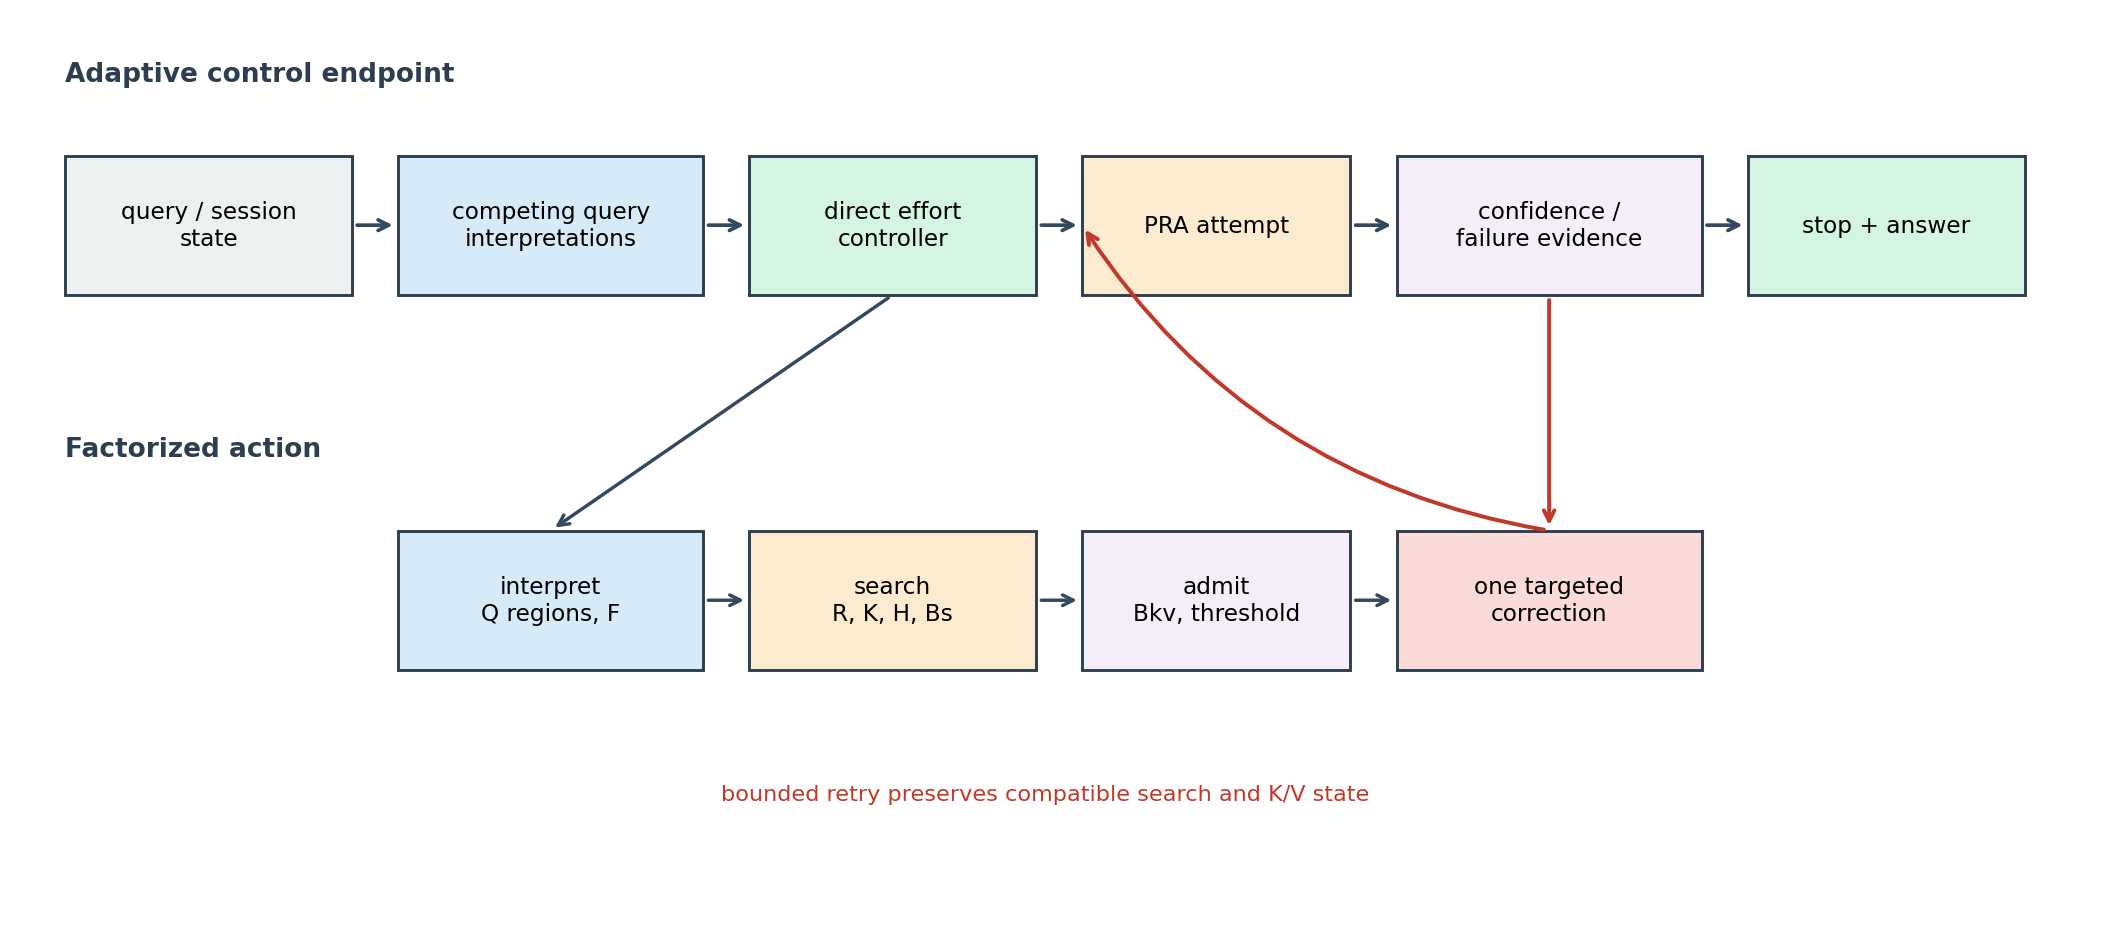
\includegraphics[width=\textwidth]{../shared/results/paper3_5_adaptive_pra/adaptive_pra_runtime_architecture.png}
\caption{The adaptive endpoint. Interpretation, search, and admission are independent controls.
Evaluation may authorize one bounded correction while preserving compatible identities and K/V.
The callback path is an experimental hook, not the default policy.}
\label{fig:architecture}
\end{figure}

\subsection{Robust profiles and factorized actions}

Table~\ref{tab:profiles} gives the validation-frozen profile ladder. The profiles are not universal
hyperparameters. They are a conservative SDK contract and a baseline against which independent
actions can be measured.

\begin{table}[H]
\centering
\small
\caption{Validation-frozen effort profiles. Lower routing thresholds allow broader closure.}
\label{tab:profiles}
\begin{tabular}{lrrrrrrrl}
\toprule
Profile & facets & $R$ & $K$ & $H$ & $B_s$ & $B_{kv}$ & $G$ & consumer layers\\
\midrule
E0 low & 1 & 1 & 2 & 0 & 2 & 256 & 256 & 27\\
E1 medium & 2 & 2 & 4 & 1 & 4 & 512 & 128 & 26--27\\
E2 high & 4 & 4 & 8 & 3 & 8 & 1024 & 64 & 24--27\\
\bottomrule
\end{tabular}
\end{table}

Profiles increase every permission together. Factorized actions do not. They can spend on roots
without buying more facets or hops, and can search broadly while admitting a compact physical set.
This flexibility creates a larger prediction problem, so oracle headroom and learned policy quality
must be reported separately.

\subsection{Accounting without unit confusion}

Let $N$ be the available candidate parents, $E$ the required evidence parents, and $K$ the admitted
parents. Evidence recall, precision, and complete recovery are
\begin{equation}
R_E=\frac{|K\cap E|}{|E|},\qquad
P_E=\frac{|K\cap E|}{|K|},\qquad
C_E=\mathbf 1[E\subseteq K].
\label{eq:evidence-metrics}
\end{equation}
$K/N$ asks what fraction of available memory was activated. $K/E$ asks how much memory was
activated per required evidence item. Neither is a latency measure.

We keep five quantities distinct: search comparisons, unique conceptual candidates searched,
conceptual candidates admitted, native K/V tokens or layer-token states, and wall-clock latency.
Collapsing them into one number would make a posting-list lookup appear equivalent to a GPU dot
product. The abstract cost used inside the factorized study is therefore an auditable ordering, not
a serving-time claim.

\section{Experimental Setup}

The primary study reuses frozen Paper-2.5 native graph and query scores. Its grouped split contains
95 validation and 65 held-out HotpotQA/QASPER example--seed units. Validation supplies targets and
thresholds; held-out oracle labels are evaluator-only. Complete evidence-chain recovery is primary.

The retrieval-representation study uses Paper-2.6's 58 validation and 74 held-out identities across
QASPER, HotpotQA, 2Wiki, and MuSiQue; 68 held-out examples contain a successor decision. The graph
and callback experiment restores the same boundary and executes all 29,700 legal actions. Eight
stratified examples check native-K/V materialization and frozen Qwen3-0.6B decode.

These scopes are not merged. The 65-unit endpoint is frozen-score chain recovery, the 74-identity
endpoint is matched-budget evidence discovery, and the eight-example endpoint is a mechanism check.
No generated-answer score is imputed for retrieval-only configurations.

Controllers may observe query features, score gaps, entropy, root competition, channel agreement,
frontier shape, and selected counts. Dataset identity, gold evidence, oracle actions, answer
correctness, and evidence recall are rejected before serving feature construction. Five seeds
measure initialization variability, not linguistic coverage.

The factorized study orders actions by
\begin{equation}
C(a)=F+N_{\mathrm{transition}}+B_s+\frac{T_{kv}}{64},
\label{eq:factorized-cost}
\end{equation}
where $T_{kv}$ is admitted source tokens. Artifacts also retain unscaled comparisons, searched and
admitted parents, K/V tokens, and wall time. The cost is an auditable within-study ordering, not a
serving-time surrogate.

\section{Factorized Control: The Main Result}

We replay
\begin{equation}
(F,R,K,H,B_s,B_{kv})\in
\{1,2,4\}\times\{1,2,4\}\times\{2,4,8\}\times
\{0,1,2,3\}\times\{2,4,8\}\times\{2,4,8\}.
\end{equation}
Actions with $B_s<R$ or $B_{kv}<R$ are invalid, leaving 792 measured configurations per unit.
Query-region policy and traversal order are fixed to isolate profile coupling.

\begin{figure}[H]
\centering
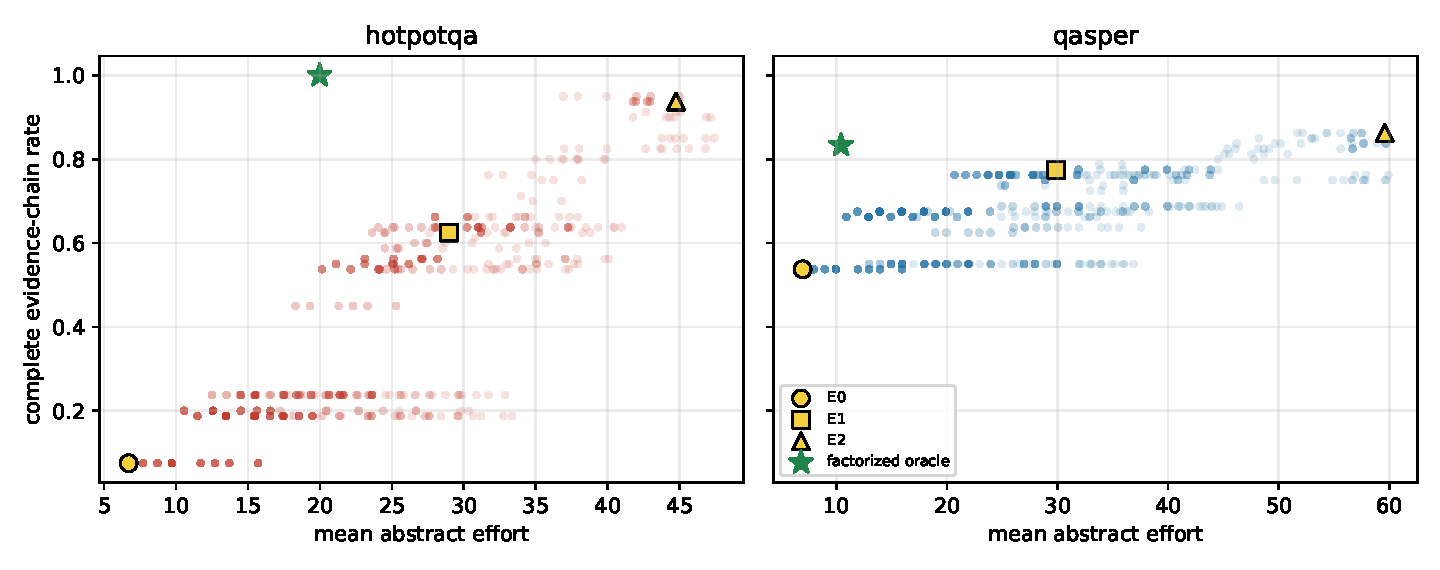
\includegraphics[width=.94\textwidth]{../shared/results/paper3_5_adaptive_pra/factorized_quality_cost_frontier.pdf}
\caption{Held-out quality--cost surface. Stars are minimum-cost factorized oracles; E0--E2 are
diagonal profile actions under the same accounting.}
\label{fig:factorized-frontier}
\end{figure}

\begin{table}[H]
\centering
\small
\caption{Profile quantization regret. Matched rows contain units solved in both spaces.}
\label{tab:factorized-oracle}
\begin{tabular}{lrrrrrr}
\toprule
Dataset & matched $n$ & profile quality & factor quality & profile cost & factor cost & regret\\
\midrule
HotpotQA & 35 & 1.000 & 1.000 & 34.18 & 19.98 & 14.20\\
QASPER matched & 24 & 1.000 & 1.000 & 16.11 & 8.95 & 7.15\\
QASPER all & 30 & .800 & .833 & 16.82 & 10.43 & ---\\
\bottomrule
\end{tabular}
\end{table}

At matched chain quality, factorization lowers mean HotpotQA cost by 41.5\% and matched QASPER cost
by 44.4\%. It also solves one QASPER unit no profile solves. Difficult examples usually need one
expensive control rather than E2 in full. One facet suffices for 97.1\% of HotpotQA and 96.7\% of
QASPER units. HotpotQA's additional work concentrates in root count, one graph hop, and parent
budget; QASPER is root-only in 96.7\% of units.

\begin{table}[H]
\centering
\small
\caption{Held-out candidate-normalized efficiency. Oracle and retry rows are evaluator ceilings;
$KV$ is mean admitted native-K/V tokens.}
\label{tab:normalized-efficiency}
\begin{tabular}{llrrrrrr}
\toprule
Dataset & Policy & $R_E$ & $P_E$ & $C_E$ & $K/N$ & $K/E$ & $KV$\\
\midrule
HotpotQA & R0 profile & .733 & .400 & .543 & .697 & 1.905 & 979\\
 & factorized oracle & .824 & .624 & .600 & .576 & 1.633 & 840\\
 & targeted retry & .948 & .476 & .886 & .756 & 2.090 & 1079\\
\addlinespace
QASPER & R0 profile & .750 & .450 & .700 & .182 & 2.267 & 636\\
 & factorized oracle & .917 & .796 & .833 & .109 & 1.550 & 431\\
 & targeted retry & .917 & .588 & .833 & .190 & 2.517 & 675\\
\bottomrule
\end{tabular}
\end{table}

QASPER supplies the cleanest sparse ceiling: the oracle raises recall and precision while admitting
fewer candidates and 205 fewer K/V tokens than R0. HotpotQA is denser at this parent granularity;
retry raises recall by activating more memory.

\begin{figure}[H]
\centering
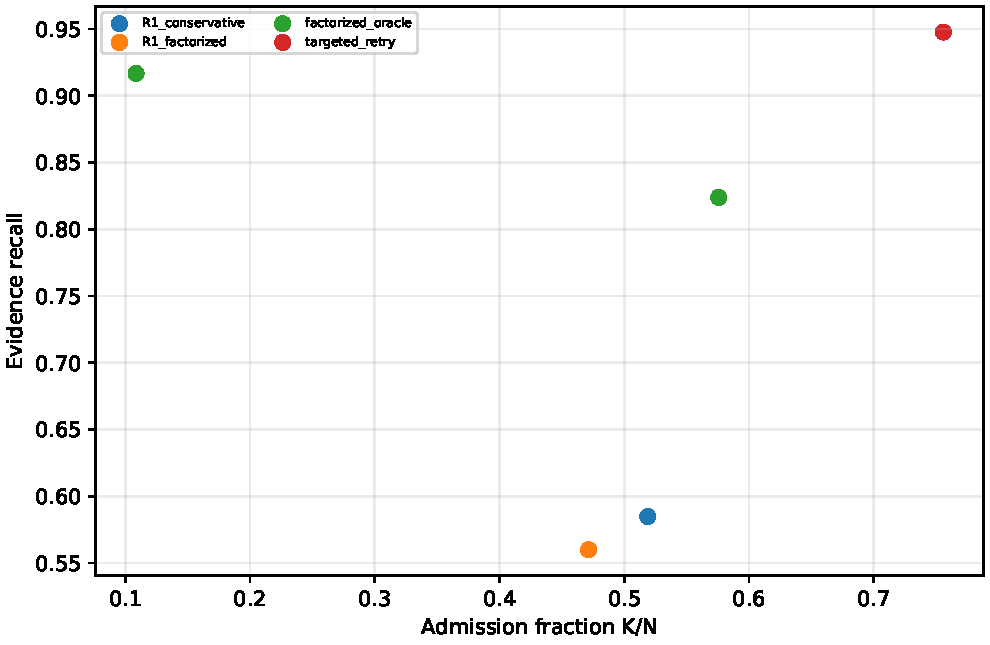
\includegraphics[width=.76\textwidth]{../shared/results/paper3_5_adaptive_pra/controller_oracle_learned_pareto.pdf}
\caption{Evidence recall against admitted candidate fraction. Learned policies below R0 save cost
by losing complete-chain quality.}
\label{fig:normalized-frontier}
\end{figure}

\section{Can We Predict the Cheap Sufficient Action?}

Oracle optimization proves cheap actions exist; it does not make them observable. R0 predicts one
profile. R1 predicts independent controls. Conservative R1 selects an upper quantile. R2 adds a
signed-hash question representation. R3A predicts controls autoregressively.

\begin{table}[H]
\centering
\small
\caption{Representative held-out factorized-target controllers. Under-allocation means missing a
chain completed by the factorized oracle.}
\label{tab:factorized-routers}
\begin{tabular}{lrrrr}
\toprule
Router & quality & cost & under & over\\
\midrule
R0 profile & .631 & 24.29 & .292 & .523\\
R1 independent & .538 & 16.13 & .385 & .378\\
R1 conservative & .560 & 17.97 & .363 & .422\\
R2 conservative & .548 & 18.06 & .375 & .400\\
R3A autoregressive & .486 & 17.18 & .437 & .335\\
Factorized oracle & .923 & 15.57 & .000 & .000\\
\bottomrule
\end{tabular}
\end{table}

\begin{figure}[H]
\centering
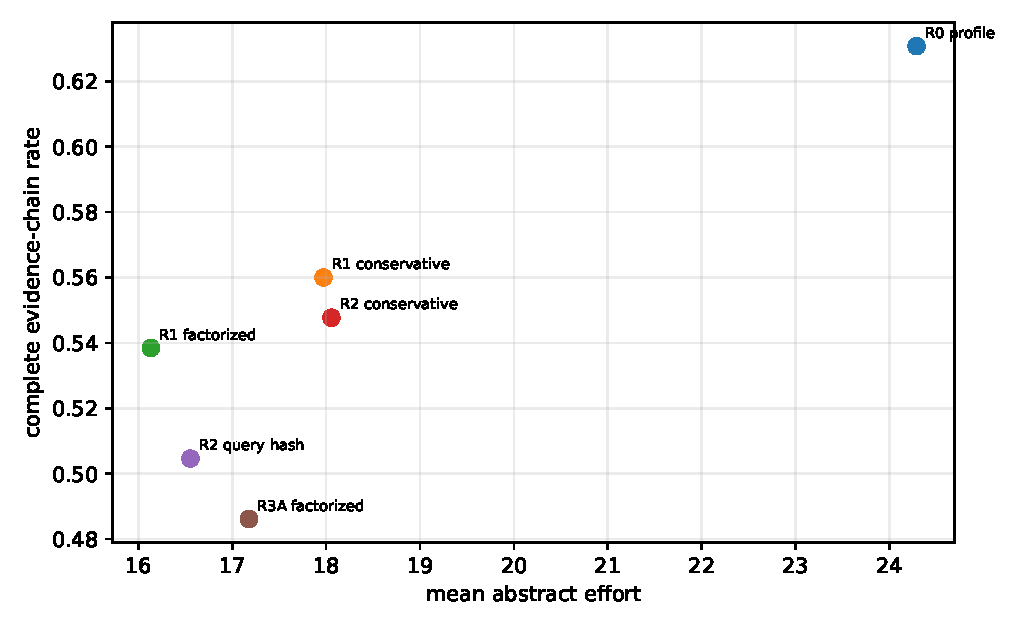
\includegraphics[width=.72\textwidth]{../shared/results/paper3_5_adaptive_pra/factorized_router_quality_cost.pdf}
\caption{Learned quality versus expected cost. Apparently cheap fine-grained policies fail to
allocate resources required by solvable examples.}
\label{fig:factorized-routers}
\end{figure}

No fine-grained router dominates R0. Conservative decoding recovers some quality over argmax, but
lower cost remains coupled to under-allocation. R0 stays the supported initial controller despite
its measurable quantization regret.

One evaluator-side retry exposes correction headroom. The cheapest successful single-control change
or compound fallback raises aggregate quality from .631 to .923 at 2.49 mean added cost, correcting
all 15 HotpotQA failures and four of nine QASPER failures without breaking a correct case. Eight
repairs change only root or facet count. This is an oracle audit, not an online policy.

Model-native query representations do not rescue the controller. Grouped validation selects the
last question-token embedding, whose held-out quality is .668 at cost 27.20, below observable
profile routing at .702 and 28.25. Deeper hidden states, native Q/K, and a 256-token contextual
diagnostic do not improve validation-selected control (Appendix~\ref{app:self-routing}).

\section{Retrieval Representation Is Also a Control Variable}

Effort asks how broadly to search; representation asks what evidence relation defines the search.
Root and successor methods independently choose semantic, exact, BM25, approximate, or hybrid
variants. A semantic root may expose an exact address, so $S_r=S_s$ is not required.

The 74 held-out root oracles choose all five representations; none has majority support. Among 68
successor-bearing examples, 22 of 25 root-to-successor pairs occur. The most frequent cell contains
only nine examples.

\begin{figure}[H]
\centering
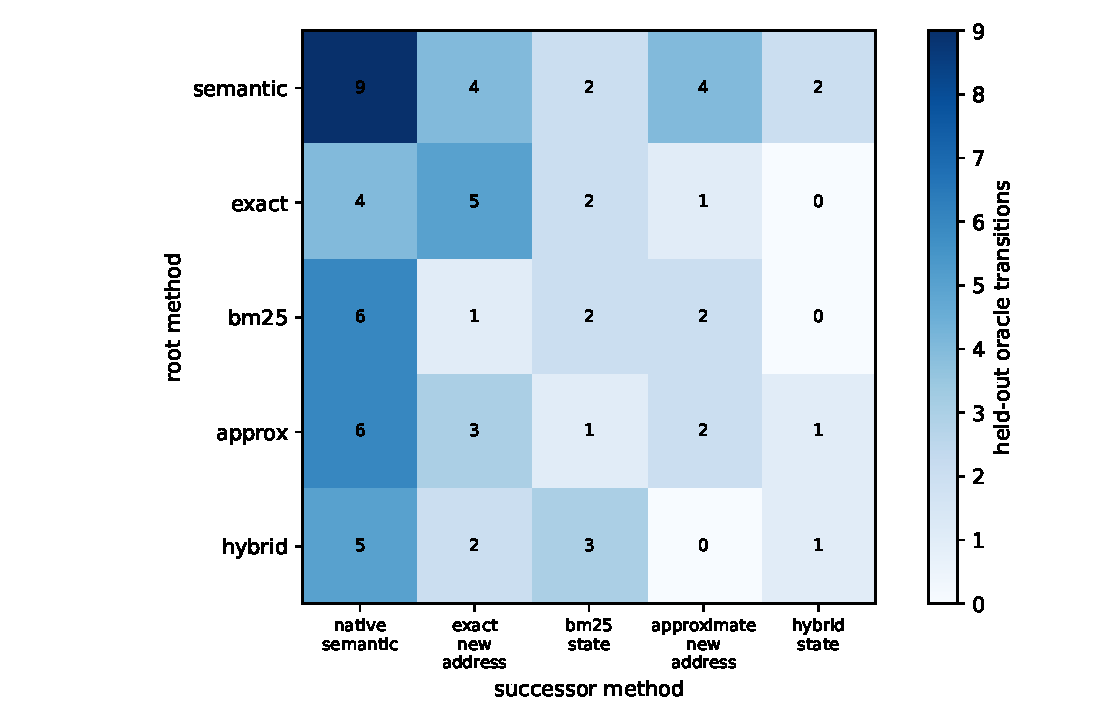
\includegraphics[width=.70\textwidth]{../shared/results/paper3_5_adaptive_pra/adaptive_search_methods/root_successor_method_heatmap.pdf}
\caption{Per-example oracle transitions justify independent root and successor actions, but do not
make the oracle observable.}
\label{fig:method-transitions}
\end{figure}

\begin{table}[H]
\centering
\small
\caption{Matched two-root plus two-successor policies over 68 held-out examples.}
\label{tab:method-policies}
\begin{tabular}{llrrr}
\toprule
Policy & interpretation & recall & precision & MRR\\
\midrule
Fixed & BM25 root, native-semantic successor & .030 & .081 & .229\\
Static hybrid & one hybrid at both stages & .035 & .088 & .229\\
Learned joint & predicted root and successor & .032 & .074 & .225\\
Interpretable cascade & gap/disagreement rules & .048 & .118 & .240\\
Per-example oracle & best measured pair & .143 & .353 & .615\\
\bottomrule
\end{tabular}
\end{table}

Representation heterogeneity is real; reliable selection is unresolved. The cascade is strongest
overall but loses to the fixed pair on QASPER and MuSiQue. Leave-one-dataset-out method accuracy is
.167--.278. Learned targeted retry raises .032 only to .037, while oracle correction reaches .143.

\section{How Far Should Adaptation Go?}

\subsection{Query interpretation}

In matched controls, explicit spans and structural query regions preserve root R@1 through 8,192
following payload tokens; a 16-token recent head fails after 32. Structural discovery is perfect on
six semi-natural fixtures but falls to .400 under five role decoys, where recent-head remains
correct. Explicit caller roles are preferred; automatic interpretations should compete under
disagreement rather than unconditionally replace one another.

\subsection{Semantic graph facets}

Request/reply supports global, syntactic, multiscale, graph, and hierarchical syntactic-to-graph
facets. Hierarchical nodes retain spans, centroids, entities, lexical and graph statistics,
confidence, and parent/child provenance. Per-facet routing supports fixed, type-rule, learned, and
oracle channel policies.

Graph facets are specialized, not universal. On the complete callback surface, the action oracle
chooses global facets for 83.8\% of examples, structural facets for 13.5\%, and graph facets for
2.7\%. Prototype graph construction costs 32--34 ms/example in exhaustive Python/CUDA replay.
Detailed quality and construction rows are in Appendix~\ref{app:graph}.

\subsection{One root-state callback}

The callback observes selected roots once and may choose a successor method or graph refinement.
It cannot inspect dataset identity, evidence, or answers. A fair comparison crosses nine facet
profiles with five root and five successor methods at the same two-root, two-successor, four-chunk
budget:
\[
132\times9\times5\times5=29{,}700\text{ actions}.
\]

\begin{table}[H]
\centering
\small
\caption{Matched test evidence recall. Learned and threshold rows report five-seed mean $\pm$
standard deviation. B6/B7 are evaluator ceilings.}
\label{tab:root-callback}
\begin{tabular}{lll}
\toprule
ID & policy & recall\\
\midrule
B0 & validation-fixed global request/reply & .205\\
B1 & query-only one-shot, no graph & $.180\pm.022$\\
B2 & query-only one-shot, graph available & $.180\pm.023$\\
B3 & root callback, no graph & $.168\pm.021$\\
B4 & root callback, graph initially available & $.167\pm.019$\\
B5 & learned conditional graph refinement & $.167\pm.021$\\
B5t & threshold graph refinement & $.188\pm.024$\\
B6 & complete-action oracle & .365\\
B7 & stage-wise oracle & .365\\
\bottomrule
\end{tabular}
\end{table}

\begin{figure}[H]
\centering
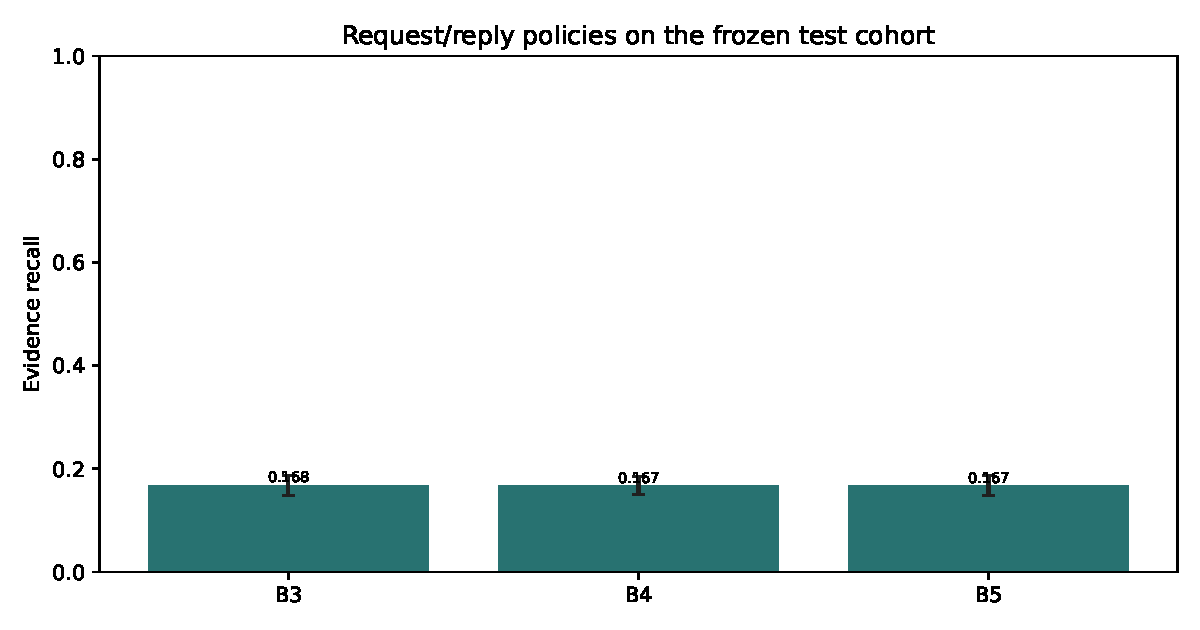
\includegraphics[width=.72\textwidth]{../shared/results/paper3_5_adaptive_pra/root_callback/controller/callback_quality.pdf}
\caption{Added root-state complexity does not improve the supported retrieval frontier. Error bars
reflect controller seeds, not example uncertainty.}
\label{fig:callback}
\end{figure}

Learned callbacks underperform matched one-shot control. Threshold refinement is somewhat better
but remains below B0 and invokes graph on 16.5\% of cases. Complete-action and stage-wise evaluator
ceilings coincide at .3649 recall, .5777 precision, .7964 MRR, and .0270 complete recovery. Thus
there is no additional stage-wise oracle advantage under these legal actions and supervision. This
does not imply post-root state can never help under different representations, actions, training,
or supervision.

\section{Native-K/V Decode Confirmation}

We map four conceptual chunks to 128 unique native-K/V tokens across Qwen layers 20--27 on two test
examples per dataset. Every memory condition exposes 1,024 token-layer states (4 MiB), averaging
7.75\% of source tokens.

\begin{table}[H]
\centering
\small
\caption{Eight-example frozen decode confirmation. $\Delta\log p$ is relative to no memory. This
is a mechanism check, not benchmark QA.}
\label{tab:decode}
\begin{tabular}{lrrrr}
\toprule
Condition & retrieval recall & exact/F1 & $\Delta\log p$ & K/V tokens\\
\midrule
No memory & .000 & .375 & .000 & 0\\
B0 fixed & .279 & .375 & +.567 & 128\\
B1 one-shot & .358 & .500 & +.770 & 128\\
B3 callback & .228 & .375 & +.912 & 128\\
B5t threshold & .360 & .500 & +.687 & 128\\
B6 oracle & .533 & .500 & +.639 & 128\\
\bottomrule
\end{tabular}
\end{table}

Every memory row improves gold-token likelihood, confirming that materialized K/V affects the
consumer. Exact/F1 is not monotonic in recall or likelihood. We therefore keep separate
\[
\text{retrieval quality}\neq\text{likelihood utility}\neq\text{generated answer quality}.
\]

\section{Discussion}

\paragraph{Lesson 1: factorization matters.}
Queries do not require one scalar effort level. Coherent profiles are robust operating points, but
they should not define the full internal action space.

\paragraph{Lesson 2: prediction is harder than optimization.}
The oracle proves cheap sufficient actions exist. Current controllers do not identify them
reliably; their lower cost is coupled to lower quality.

\paragraph{Lesson 3: more adaptation is not automatically better.}
Representation choices, graph facets, and callbacks enlarge the capability surface without
producing a better learned deployable frontier. These negative results stop open-ended complexity.

\paragraph{Lesson 4: preserve optionality.}
Independent actions and one bounded callback hook remain useful architectural options because
PRA-aware training may change the geometry. The supported frozen runtime remains conservative:
explicit query roles, R0 initial effort, validation-fixed request/reply, independent budgets,
observable traces, and at most one correction.

\section{Related Work}

\paragraph{External and iterative retrieval.}
RAG and DPR retrieve external text~\cite{lewis2020rag,karpukhin2020dpr}. MDR, IRRR, and IRCoT make
retrieval state dependent~\cite{xiong2021mdr,qi2021irrr,trivedi2023ircot}. Adaptive-RAG selects no,
single, or iterative retrieval~\cite{jeong2024adaptiverag}; FLARE retrieves during generation
~\cite{jiang2023flare}; Self-RAG trains retrieval and reflection decisions~\cite{asai2024selfrag}.
PRA instead controls query representation, persistent identity traversal, and native-K/V admission.

\paragraph{K/V selection and sparse attention.}
H2O, SnapKV, StreamingLLM, Quest, KIVI, and ClusterKV select, index, evict, or compress physical K/V
~\cite{zhang2023h2o,li2024snapkv,xiao2023streamingllm,tang2024quest,liu2024kivi,liu2024clusterkv}.
PagedAttention manages storage~\cite{kwon2023vllm}. PRA separates upstream logical discovery from
physical activation; paging, compression, and eviction remain complementary.

Longformer, BigBird, Reformer, and Routing Transformer change architectural sparsity
~\cite{beltagy2020longformer,zaheer2020bigbird,kitaev2020reformer,roy2021routing}. RETRO,
Memorizing Transformers, Compressive Transformer, Infini-Attention, Landmark Attention, and Titans
provide external, recurrent, compressed, or learned memory~\cite{borgeaud2022retro,wu2022memorizing,
rae2020compressive,munkhdalai2024infini,mohtashami2023landmark,behrouz2025titans}. We do not imply
equivalence to a frozen PRA control layer.

\paragraph{Adaptive computation.}
Adaptive Computation Time learns halting~\cite{graves2016adaptive}; early exit allocates depth
~\cite{xin2020deebert}; sparse experts allocate parameters~\cite{fedus2022switch}; and
Mixture-of-Depths allocates layer compute across tokens~\cite{raposo2024mixturedepths}. PRA controls
a different object: interpretation, retrieval representation, traversal, and K/V disclosure, whose
costs cannot be reduced to one uniform operation count.

\section{Limitations}

The primary endpoint is frozen-score chain recovery, not generated answer quality; the live decode
check has eight examples. The factorized cohort has 65 held-out example--seed units but only 32
unique questions. The channel study has 74 held-out identities and 68 successor labels. Five seeds
do not replace larger identity cohorts or cross-model replication.

Equation~\ref{eq:factorized-cost} orders actions within this study. Python/CUDA graph timings and
inherited CPU systems measurements are not production latency. Automatic query interpretation is
heuristic. Learned controllers use small validation sets; strong retry and action oracles use
evaluator outcomes and cannot be deployed.

The callback surface fixes two roots, two successors, and four admitted chunks. It does not cross
hop depth, variable admission, or jointly trained root-state representations. Equal complete and
stage-wise ceilings apply only to this Cartesian surface. No PRA-aware backbone is trained here.

\section{Conclusion}

\paragraph{What did we learn?}
Factorized controls expose cheaper sufficient PRA actions: HotpotQA cost falls from 34.18 to 19.98
and matched QASPER from 16.11 to 8.95 at matched chain quality.

\paragraph{What did not work?}
Fine-grained routers, model-native self-routing, learned representation selection, graph control,
and callbacks do not beat the robust conservative policy. Their oracle headroom is real; their
observable prediction is not reliable enough.

\paragraph{What follows?}
Paper 4 studies PRA-aware training, Paper 5 scaling, Paper 5.5 runtime productization, and Paper 6
first-class vLLM integration. This paper closes frozen adaptive inference with a factorized action
space, a conservative default, and a clear stopping point for controller complexity.

\appendix

\section{Query-Region Diagnostics}
\label{app:query-regions}

The matched corpus crosses 24 cases, three payload forms, and five serializations while holding
evidence, eight candidate roots, and 16 active K/V tokens fixed.

\begin{table}[H]
\centering
\scriptsize
\caption{Root R@1 / answer proxy under matched layouts.}
\begin{tabular}{lcccc}
\toprule
Layout & recent head & explicit & structural & head+reinterpret\\
\midrule
$C+Q$ & 1.00/1.00 & 1.00/1.00 & 1.00/1.00 & 1.00/1.00\\
$Q+C$ & .00/.00 & 1.00/1.00 & 1.00/1.00 & 1.00/1.00\\
$C_1+Q+C_2$ & .00/.00 & 1.00/1.00 & 1.00/1.00 & 1.00/1.00\\
$I+C+Q$ & 1.00/1.00 & 1.00/1.00 & 1.00/1.00 & 1.00/1.00\\
$Q+$long payload & .00/.00 & 1.00/1.00 & 1.00/1.00 & 1.00/1.00\\
\bottomrule
\end{tabular}
\end{table}

Head R@1 averages .400; explicit and structural average 1.000. Reinterpretation corrects all 216
head failures and breaks none of 144 correct cases. Broad all-region selection reaches .333.

\begin{figure}[H]
\centering
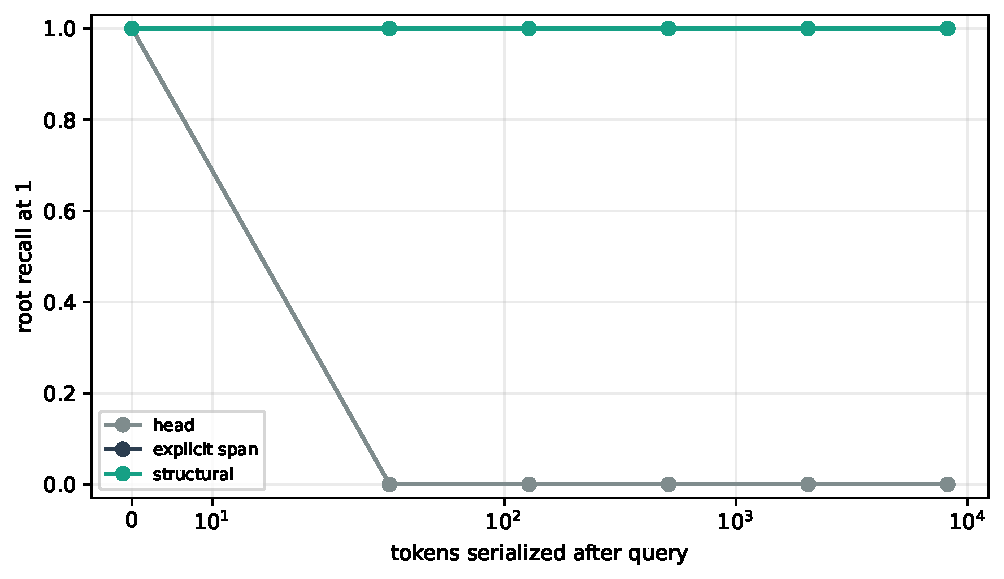
\includegraphics[width=.70\textwidth]{../shared/results/paper3_5_adaptive_pra/query_region_displacement.pdf}
\caption{Recent-head failure under displacement; explicit and structural spans remain stable.}
\end{figure}

Structural discovery reaches R@1 1.000 and span IoU .981 on six semi-natural fixtures. Under five
role decoys, it falls to .400 and .314. Session, region-count, facet, URL-role, and retry details
remain in the artifacts.

\section{Preliminary Profile-Derived Routers}

\begin{table}[H]
\centering
\small
\caption{Held-out routers trained on inherited profile labels.}
\begin{tabular}{lrrrr}
\toprule
Router & quality & cost & under & over\\
\midrule
R0 profile & .615 & 109.9 & .031 & .169\\
R1 feature MLP & .594 & 103.7 & .055 & .166\\
R2 signed-hash MLP & .591 & 104.0 & .046 & .157\\
R3A autoregressive & .591 & 102.6 & .049 & .145\\
\bottomrule
\end{tabular}
\end{table}

These labels inherit profile coupling and are superseded by the factorized-target experiment. Added
capacity saves nominal cost while losing quality.

\section{Self-Encoded Query Routing}
\label{app:self-routing}

Qwen3-0.6B is frozen at revision
\texttt{c1899de289a04d12100db370d81485cdf75e47ca}. The sweep pools the explicit question span from
embeddings, hidden layers, and pre-RoPE native Q/K. Projection and selection use grouped validation.

\begin{table}[H]
\centering
\small
\caption{Representative five-seed profile routing by representation.}
\begin{tabular}{lrrrr}
\toprule
Representation & CV quality & test quality & total cost & under\\
\midrule
Observables & .728 & .702 & 28.25 & .222\\
Signed hash & .686 & .609 & 25.53 & .314\\
Embedding last (selected) & .726 & .668 & 27.20 & .255\\
Embedding mean & .699 & .717 & 25.74 & .206\\
Hidden layer 7 mean & .714 & .698 & 27.13 & .225\\
Native K layer 13 mean & .718 & .655 & 27.85 & .268\\
Contextual layer 14 mean & .705 & .674 & 27.70 & .249\\
\bottomrule
\end{tabular}
\end{table}

Embedding mean is numerically highest on test but was not validation-selected. Contextual states
cost more and do not improve selected control. Exact prefix continuation before the first PRA
consumer reuses the state without changing quality.

\section{Inherited Runtime and Proxy Measurements}

These are provenance for Paper 5.5, not Paper 3.5 contributions. At 4,096 keys, exact GEMM reduces a
Python Top-8 loop from .827 s to .327 ms with parity. The coarse index reaches .332--.648 recall and
takes 8--13 ms, so it is not adopted. CPU gather shows no stable speed advantage; Python page lookup
is 14--37 times slower. At concurrency 32, padding wastes 44.1\% of slots. None is a production GPU
throughput result.

The controlled 1,024-document, 200-query corpus forces a two-hop bridge. One-shot RAG and fixed low
PRA recover .005; iterative RAG and adaptive medium PRA recover 1.000 with controlled active-token
counts 320 and 192. The construction demonstrates accounting and iteration, not general superiority.
Mechanism-faithful K/V proxy rows are likewise retained as bookkeeping controls, not system rankings.

\section{Graph Diagnostics}
\label{app:graph}

\begin{table}[H]
\centering
\small
\caption{Global graph versus hierarchical syntactic-to-graph root discovery.}
\begin{tabular}{lrrrrrr}
\toprule
Dataset & graph R & hier. R & graph work & hier. work & graph ms & hier. ms\\
\midrule
QASPER & .033 & .064 & 90 & 90 & 31.9 & 18.8\\
HotpotQA & .234 & .212 & 524 & 524 & 70.2 & 35.5\\
2Wiki & .175 & .175 & 288 & 288 & 40.1 & 31.1\\
MuSiQue & .090 & .092 & 796 & 570 & 39.1 & 36.1\\
\bottomrule
\end{tabular}
\end{table}

Adding graph to inherited hybrid changes recall by -.0078, +.0156, zero, and -.0078 on QASPER,
HotpotQA, 2Wiki, and MuSiQue. Per-facet fixed, type-rule, learned, and oracle policies reach .120,
.224, $.198\pm.020$, and .283 recall on an explicitly post-hoc exploratory split. Graph calls,
density, components, overlap, and facet assignments remain public.

\section{Callback Ablations}

Adding the root gist raises learned B5 recall from .167 to .177, still below B1. Threshold control
corrects 21.6\% and harms 17.6\%; three of five seeds invoke no graph. Leave-one-dataset-out B1, B2,
B3, and B5t reach .167, .170, .155, and .180 versus .190 fixed and .365 oracle. Full seed behavior,
feature ablations, correction/harm rows, and transfer tables remain in the result package.

\section{SDK and Artifact Manifest}
\label{app:artifacts}

An independent implementation should preserve five invariants: separate conceptual and physical
budgets; reject evaluator labels before vectorization; reuse compatible identity and K/V state while
accounting for regeneration; label component versus end-to-end timing; and keep query-role discovery
separate from faceting with explicit caller spans authoritative.

Core contracts are in \path{src/pra_hf/adaptive_runtime.py},
\path{src/pra_hf/factorized_control.py}, \path{src/pra_hf/adaptive_search.py},
\path{src/pra_hf/adaptive_facets.py}, \path{src/pra_hf/facet_routing.py}, and
\path{src/pra_hf/root_callback.py}. Drivers under \path{experiments/paper3_5_adaptive_pra} generate
the profile, factorized, normalized-efficiency, self-router, graph, callback, and decode artifacts.

All normalized outputs are under
\path{docs/papers/shared/results/paper3_5_adaptive_pra}. They include identity partitions, action
specifications, controller seeds, calibration, oracle and Pareto rows, allocation outcomes,
candidate/KV accounting, graph construction and overlap, callback ablations, decode rows, findings
JSON, plots, and claim audits. The 29,700-action surface and 5,940 persisted root states support
policy replay without repeating retrieval. The README lists complete study commands.

\small
\bibliographystyle{plain}
\bibliography{../shared/references}
\end{document}
